\documentclass[xcolor={dvipsnames}]{beamer}

\usepackage{fontspec}

\usetheme{metropolis}

\usepackage{subcaption}
\usepackage{mathtools}
\usepackage{amssymb,amsfonts}
\usepackage{dsfont,mathrsfs}


\usepackage{hyperref,cleveref}
\usepackage{graphicx}
\usepackage{enumitem}

\setlist{itemsep=0pt,topsep=0pt}

\usepackage{csquotes}
\usepackage[
	sorting=none,
	minnames=1,
	maxcitenames=2,
	backend=biber
]{biblatex}

\addbibresource{../bibliography/references.bib}


%% Hyperref %%


%%% DEFINE MACROS %%%

%% Math %%

\newcommand{\RR}{\mathbb{R}}
\newcommand{\TT}{\mathbb{T}}
\newcommand{\QQ}{\mathbb{Q}}
\newcommand{\NN}{\mathbb{N}}
\newcommand{\BB}{\mathbb{B}}
\newcommand{\WW}{\mathbb{W}}
\newcommand{\EE}{\mathbb{E}}
\newcommand{\PP}{\mathbb{P}}

\newcommand{\bfR}{\mathbf{R}}
\newcommand{\bfP}{\mathbf{P}}


\newcommand{\calC}{\mathcal{C}}
\newcommand{\calE}{\mathcal{E}}
\newcommand{\calI}{\mathcal{I}}
\newcommand{\calH}{\mathcal{H}}
\newcommand{\calK}{\mathcal{K}}
\newcommand{\calL}{\mathcal{L}}
\newcommand{\calP}{\mathcal{P}}
\newcommand{\calO}{\mathcal{O}}
\newcommand{\calT}{\mathcal{T}}
\newcommand{\calS}{\mathcal{S}}
\newcommand{\calM}{\mathcal{M}}
\newcommand{\calW}{\mathcal{W}}
\newcommand{\calX}{\mathcal{X}}

\newcommand{\suchthat}{\text{s.t.}}

\renewcommand{\phi}{\varphi}
\renewcommand{\epsilon}{\varepsilon}

\DeclareMathOperator{\divg}{div}
\DeclareMathOperator{\Ent}{Ent}
\DeclareMathOperator{\supp}{supp}
\DeclareMathOperator*{\argmin}{argmin}
\DeclareMathOperator*{\argmax}{argmax}

\DeclareMathOperator{\KL}{KL}
\DeclareMathOperator{\proj}{proj}
\DeclareMathOperator{\prox}{prox}

%\numberwithin{equation}{section}

%% Colors %%

\colorlet{lightblue}{RoyalBlue!13!white}
\colorlet{midblue}{RoyalBlue!70}
\colorlet{midgreen}{OliveGreen!65}
\colorlet{darkred}{Red!90!Black}

\newcommand{\redfont}{\color{darkred}}
\newcommand{\bluefont}{\color{RoyalBlue}}
\newcommand{\greenfont}{\color{Green!90!black}}


%% TITLE, AUTHOR %%

\author{
	Wilson Jallet\\
	\textit{École polytechnique, ENS Paris-Saclay}
}
\title{A regularized Optimal Transport formulation for variational Mean-Field Games}

\begin{document}

\maketitle

\section{Mean-field Games}

\begin{frame}[allowframebreaks]{The MFG problem}
	
	Introduced by \textcite{LASRY2006619,LASRY2006679} to model and study large-scale games with many agents and their Nash equilibria.
	
	\textbf{Agent dynamics:}
	\begin{equation}
		dX_t = \alpha_t dt + \sigma dW_t
	\end{equation}
	\textbf{Control objective:}
	\begin{equation}
		\inf_\alpha~
		\EE\left[
		\int_0^T \frac{1}{2}|\alpha_t|^2 + f(X_t, \rho_t) \, dt + g(X_T, \rho_T)
		\right]
	\end{equation}
	
	\framebreak
	
	\textbf{Nash equilibrium} PDEs arise from dynamic programming (see \textcite{LASRY2006679}):
	\begin{subequations}
	\begin{align}
		-\partial_t u - \frac{\sigma^2}{2}\Delta u + \frac{1}{2}|\nabla u|^2 &= f(x, \rho_t) \\
		\partial_t \rho_t - \frac{\sigma^2}{2}\Delta \rho_t - \divg(\rho_t \nabla u) &= 0 \\
		u(T, x) &= g(x, \rho_T)
	\end{align}
	\end{subequations}
\end{frame}


\begin{frame}[allowframebreaks]{Variational formulations}
	
	\textcite{benamou:hal-01295299,benamou2018entropy} consider \textit{potential games} where
	\[
		g(x,\mu) = DG(\mu), \quad
		f(x,\mu) = DF(\mu)
	\]
	for some functionals $F,G: \calP(\Omega) \to \RR$.
	
	They introduce an \textbf{Eulerian formulation:}
	\begin{subequations}
	\begin{align}
		&\inf_{\rho,v}~
		\frac{1}{2}\int_0^T \int_\Omega |v|^2 d\rho_t \, dt +
		\int_0^T F(\rho_t) \, dt +
		G(\rho_T) \\
		\text{s.t.} \quad & \partial_t \rho_t -\frac{1}{2}\Delta\rho_t + \divg(\rho_t v) = 0
	\end{align}	
	\end{subequations}

	\framebreak
	
	
	\citeauthor{benamou:hal-01295299,benamou2018entropy} introduce \textbf{Lagrangian formulations:} work with measure on space of paths $\calX = C([0,T], \RR^d)$ to minimize weighted energy.
	
	\textbf{Note:} Framework of \textcite{benamou2018entropy} works on $\Omega = \RR^d$.
	
	\textbf{Energy:} Relative entropy:
	\[
		H(q|r) = \begin{cases}
		\int_\calX \log(dq/dr)\, dq &\mbox{if } q \ll r  \\
		+\infty &\mbox{otherwise}
		\end{cases}
	\]
	
	\framebreak
	
	Solve problem
	\begin{equation}
		\inf_{Q \in \calP(\calX)}
		H(Q|R_\epsilon) + 
		\int_0^T F(Q_t) \,dt +
		G(Q_T)
		\quad \text{s.t.}\ Q_0 = \rho_0
	\end{equation}
	where $Q_t = (e_t)_\# Q$, and $R_\epsilon$ \textbf{Wiener measure} $\leftrightarrow$ law of Brownian motion of variance $\epsilon = \sigma^2$.
	
	
\end{frame}


\section{Discretization and Algorithms}

\begin{frame}{Discretization}
	
	\textbf{Time discretization.} \citeauthor{benamou2018entropy} introduce the time-discretized problem
	\begin{subequations}\label{eq:TimeDiscretePrimal}
	\begin{align}
		&\inf_\gamma~
		H(\gamma | R^N_\epsilon) +
		h \sum_{k=1}^{N} F(\rho_k) +
		G(\rho_N)  \\
		\suchthat\ & \pi^k_\#\gamma = \rho_k
	\end{align}
	\end{subequations}
	where
	\[
		R^N_\epsilon = \prod_{i<N} P_{t_{i+1}-t_i}(x_{i+1}-x_i)
	\]
	is the $N$-marginal of the Wiener measure and $P_t(z) = e^{-|z|^2/(2t)}$ is the \textbf{heat kernel} on $\RR^d$.
	
\end{frame}

\begin{frame}[allowframebreaks]{Kantorovitch potentials}
	
	Using duality, solution of \eqref{eq:TimeDiscretePrimal} is
	\begin{align*}
		\gamma^* &= \exp(\oplus_k u^*_k) R^N_\epsilon  \\
		(\rho_k^*)_{i_k} &= \sum_{j\neq k}\sum_{i_j} \gamma^*_{i_0,\ldots,i_N}
	\end{align*}
	where the potentials $u^*_k$ solve the dual problem of \eqref{eq:TimeDiscretePrimal}.
	
	\framebreak
	
	They satisfy a \textbf{fixed point condition}
	\begin{equation}
		e^{u^*_k} = \frac{
			\prox^{\KL}_{F_k}(\calI_k^*)
		}{
			\calI_k^*
		}
	\end{equation}
	where $\calI_k$ is the marginalization
	\begin{equation*}
		\calI_k(x_k) = \int_{(\RR^d)^N}
		\exp\left(\sum_{j\neq k} u_j(x_j) \right) R^N(x_0,\ldots,x_N)\, d\boldsymbol{x}_{-k}
	\end{equation*}
	
	
	
\end{frame}


\begin{frame}{Spatial discretization}
	Article by \textcite{benamou2018entropy} does not go into much detail.
	\begin{itemize}
		\item[\textbullet] define grid of size $M$ for domain $\Omega$
		\item[\textbullet] discretize kernel $R^N_\epsilon$ as tensor $\bfR$
		\item[\textbullet] replace integral with sum
	\end{itemize}
	
	\pause\textbf{\redfont Several problems:}
	\begin{itemize}
		\item[\textbullet] framework of paper works on infinite domain $\RR^d$ $\rightarrow$ how to handle finite $\Omega$?
		\item[\textbullet] integral $\calI_k$ becomes \textit{large} sum over multi-index $(i_0,\ldots,i_N)$
		\[
			\sum_{i_0,\ldots,i_N} \bfR_i \prod_{s=0}^N a_{i_s}
		\]
		\begin{itemize}
			\item[$\rightarrow$] \redfont complexity $\calO(M^N)$
		\end{itemize}
	\end{itemize}
	
\end{frame}

\begin{frame}
	Handling finite domain $\rightarrow$ for instance $\Omega = [0,1]^2$ and cut-off kernel $\bfR$ (implied in article).
	{\redfont $\rightarrow$ might be insufficient}
	
	Large sum-product: exploit structure of Wiener measure $\bfR$
	\[
		\bfR_i = \prod_{k<N} P_h(x_{i_{k+1}} - x_{i_k})
	\]\pause
	\begin{itemize}
		\item[$\rightarrow$] use \textbf{sum-product algorithm}
		\[
		\sum_{j\neq k}\sum_{i_j} \bfR_i \prod_{s=0}^N a_{i_s} =
		\mathbf{A}_{i_k} \mathbf{B}_{i_k}
		\]
		where $\mathbf{A} = \bfP^T(a_{k-1} \odot \bfP^T(a_{k-2}\odot\cdots))$ and $\mathbf{B} = \bfP(a_{k+1} \odot \bfP (a_{k+2}\odot\cdots))$
		\item[$\rightarrow$] {\boldmath\bfseries\greenfont complexity reduced to $\calO(NM^3)$!}
	\end{itemize}
\end{frame}

\begin{frame}
	\textbf{Total algorithm complexity:} 
	\[
		\calO(K N^2 M^3)
	\]
	where $K$ is number of Sinkhorn iterates. If $\bfP$ can be factorized over $\RR^d$ $\rightarrow$ get further speedup.
	
\end{frame}


\section{Numerical results}

\begin{frame}{Implementation}
	
	Built a full implementation in Python \& Cython\footnote{\url{https://github.com/ManifoldFR/mva-optimaltransport/tree/master/project}}.
	
	To measure convergence, we use the \textbf{\bluefont Hilbert metric} between two iterates $a^{(n)}$ and $a^{(n+1)}$
	\begin{equation}
		d_{N,\calH}(a^{(n)}, a^{(n+1)}) =
		\sum_{k=0}^{N}
		d_\calH(a_k^{(n)}, a_k^{(n+1)})
	\end{equation}
	where $d_\calH(u, v) = \| \log(u) - \log(v)\|_V$, $\|z\|_V = \max(z) - \min(z)$.
	
	\textbf{Separable heat kernel:} Sinkhorn iterates run in time
	\[
		\calO(KN^2 M^{3/2})
	\]
\end{frame}


\begin{frame}[allowframebreaks]{Crowd motion}
	
	Enforce hard congestion constraint $\rho \leq \bar{m}$ on agent distributions.
	
	Handling obstacles $\rightarrow$ to keep $\Omega$ convex enforce constraint $\rho = 0$ on set of obstacles $\mathscr{O}$
	
	Target set: penalize distance $\Psi$ to target with $\langle \Psi, \mu\rangle$.
	
	\textbf{Penalty:}
	\begin{align*}
		G(\mu) = \langle \Psi, \mu\rangle + \imath_{[0,\bar{m}]}(\mu) + \imath_0(\mathds{1}_\mathscr{O}\mu).
	\end{align*}
	$F$ is identical but without $\Psi$ term.
	
	$\KL$-projections have closed-form expressions.
	
	\framebreak
	
	Design $\Psi$ to be shortest-time distance to target\\
	$\rightarrow$ solution of Eikonal equation $|\nabla u(x)| = 1/f(x)$.
	
	\begin{figure}
		\centering
		\begin{subfigure}{.45\linewidth}
			\includegraphics[width=\linewidth]{../project/images/multimarg_room1/room_setup.pdf}
		\end{subfigure}~
		\begin{subfigure}{.49\linewidth}
			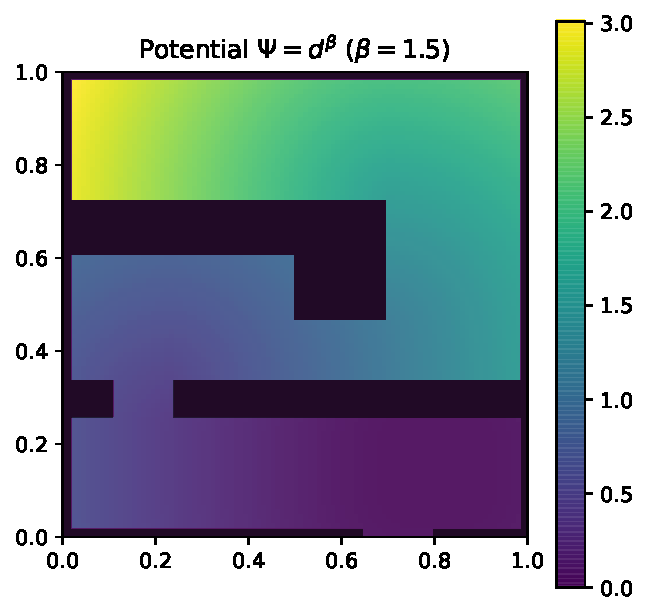
\includegraphics[width=\linewidth]{../project/images/multimarg_room1/room_potential.pdf}
		\end{subfigure}
	\end{figure}
	
\end{frame}


\begin{frame}
	
	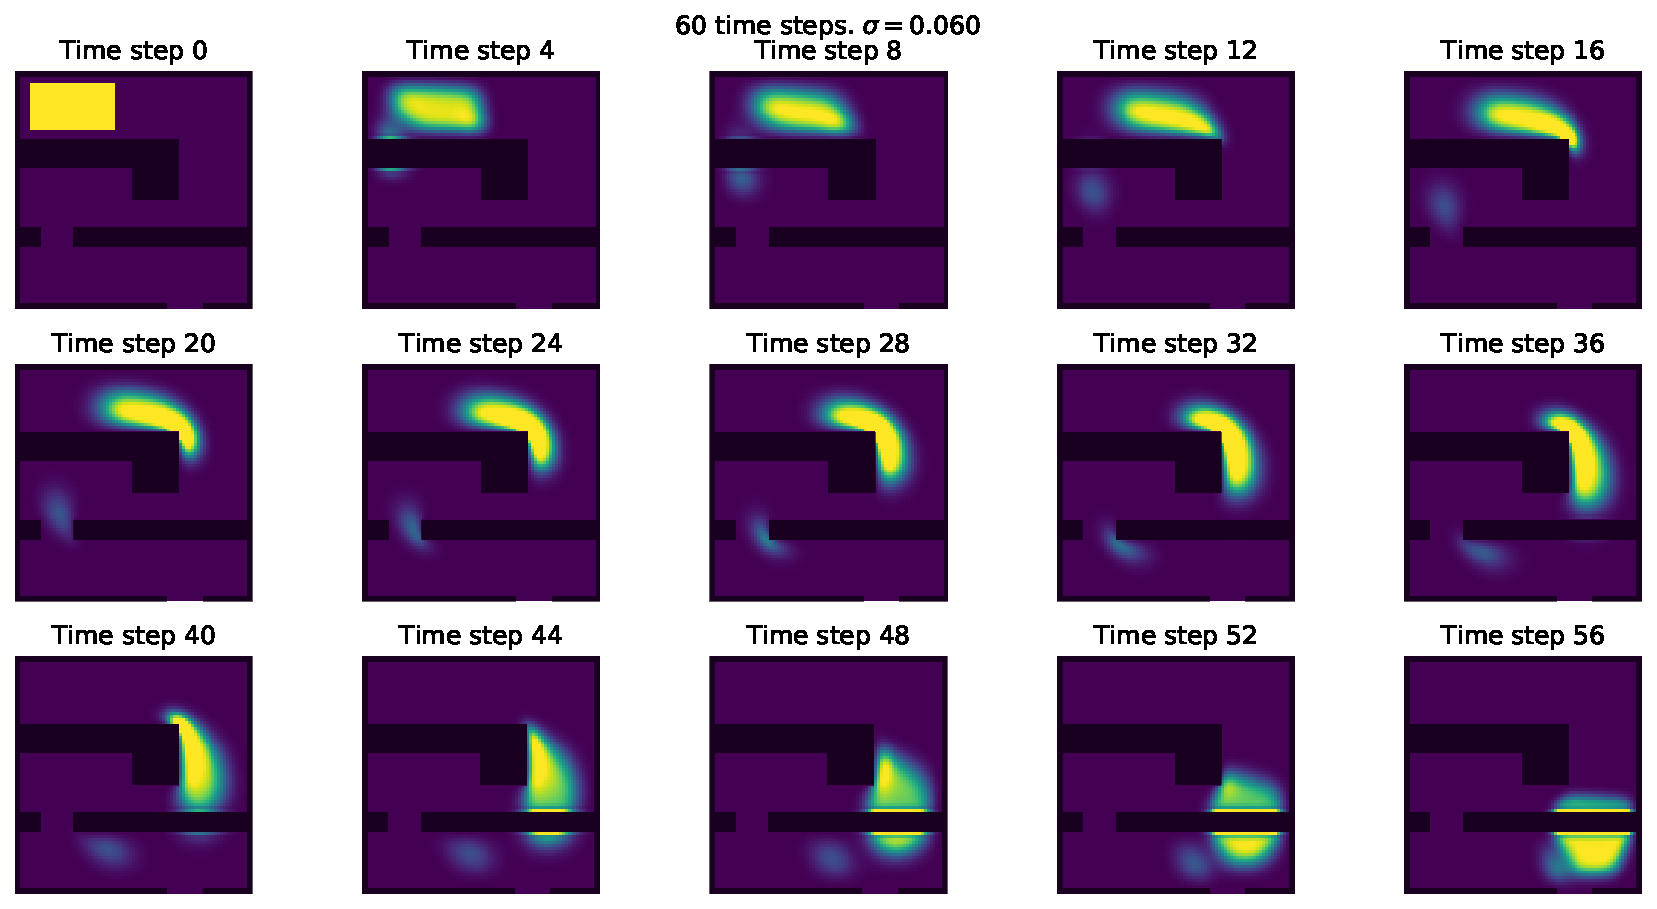
\includegraphics[width=\linewidth]{../project/images/multimarg_room1/multimarg_transport.pdf}
	Grid $M=101^2$. Convergence threshold $\eta = 10^{-8}$. CPU time: $\sim 13$ seconds.
\end{frame}

\begin{frame}
	\begin{figure}
		\centering
		\includegraphics[height=\textheight]{../project/images/multimarg_room1/hilbert_convergence.png}
		\caption{Linear convergence speed of the Hilbert metric.}
	\end{figure}
	
\end{frame}

\begin{frame}
	
	More complex domain topology:
	
	\begin{figure}
		\begin{subfigure}{.45\linewidth}
			\includegraphics[width=\linewidth]{../project/images/multimarg_room3/room_setup.pdf}
		\end{subfigure}~
		\begin{subfigure}{.49\linewidth}
			\includegraphics[width=\linewidth]{../project/images/multimarg_room3/room_potential.pdf}
		\end{subfigure}
	\end{figure}
	
\end{frame}


\begin{frame}
	\begin{figure}
	\includegraphics[width=\linewidth]{../project/images/multimarg_room3/multimarg_transport.pdf}
	\caption{Grid $M=101^2$. Convergence threshold $\eta = 10^{-8}$. CPU time: $\sim 16$ seconds.
	{\bfseries\redfont Qualitatively not terrible.}}	
	\end{figure}
\end{frame}


\begin{frame}{Analysis of results}
	
	Computational time is \textit{\greenfont very good}: Hilbert metric converges in $K = \calO(|{\log(\eta)}|)$ iterations and CPU time low.
	
	Last results are \textbf{problematic}: the agent mass ``ghosts" through the domain boundary.\\
	$\rightarrow$ maybe \textbf{use other kernel}?
	
\end{frame}

\section{Conclusion and further work}


\begin{frame}{Possible extension}
	
	
	\textbf{Suggestion:} change heat kernel $\bfP$ to something appropriate for non-convex $\Omega$ or Riemannian manifolds based on geodesic distance. See \textcite{peyr2015entropic}.
	
	Geodesic kernel $\boldsymbol{\xi}$ on $\calM$ operates as
	\[
		\boldsymbol{\xi}x =
		\left(I - \frac{s}{L}\hat{\Delta}_\calM \right)^{-L}x
	\]
	where $\hat{\Delta}_\calM$ discrete Laplacian on $\calM$, $s>0$ integration time and $L$ number of step.\\
	Typically \textbf{not} separable $\rightarrow$ {\redfont expect slower computation}\ldots
	
	\textbf{Tests} with parameters $L=10$ and $s=0.01$
	
\end{frame}


\begin{frame}
	\begin{figure}
		\includegraphics[width=.84\linewidth]{../project/images/geodesic_room3/transport.pdf}
		\caption{Application to the more complex room 2. Threshold $\eta = 10^{-3}$. CPU time: $30$ seconds. Relative $L^\infty$ constraint err $\sim 10^{-4}$. {\greenfont\bfseries Much better.}}
	\end{figure}
\end{frame}

\begin{frame}
	\begin{figure}
		\centering
		\includegraphics[width=.75\linewidth]{../project/images/geodesic_room3/congestion_plot.pdf}
		\caption{Congestion plot for room 2 w/ geodesic kernel.\\
		$\rightarrow$ Max agent density oscillates (intuitive property!)}
	\end{figure}
\end{frame}
	

\begin{frame}{Conclusion}
	
	Theoretical justification for geodesic heat kernel? Does it replace Euclidean Wiener measure on $C([0,T], \RR^d)$?
	\begin{itemize}
		\item[$\rightarrow$] do results of \textcite{benamou2018entropy} extend?
		\item[$\rightarrow$] \textbf{\bluefont extend theoretical framework to manifolds}
		\item[$\rightarrow$] fine-tune parameters $L$ and $s$?
	\end{itemize}
	\pause
	
	\textbf{Other kinds of problems} not covered: non-quadratic Hamiltonians, optimal time problems\ldots~$\rightarrow$ require Lagrangian formulations
	
\end{frame}



\begin{frame}[allowframebreaks]	
	\printbibliography{}
\end{frame}


\end{document}

